% !TeX encoding = UTF-8
% !TeX program = pdflatex
% !BIB program = biber



\documentclass[english]{lni}
\usepackage{wrapfig}
\addbibresource{festival_paper.bib}
\usepackage{pifont}% http://ctan.org/pkg/pifont
\newcommand{\cmark}{\ding{51}}%
\newcommand{\xmark}{\ding{55}}%
\begin{document}
%%% Mehrere Autoren werden durch \and voneinander getrennt.
%%% Die Fußnote enthält die Adresse sowie eine E-Mail-Adresse.
%%% Das optionale Argument (sofern angegeben) wird für die Kopfzeile verwendet.
\title[To Pump or Not to Pump]{To Pump or Not to Pump - Sensor-based Reinforcement
Learning for an Optimal Scheduler}
%% \subtitle{Untertitel / Subtitle} % if needed
\author[1]{Alissa Müller}{almueller@techfak.uni-bielefeld.de}{0009-0009-3731-8665}
\author[1]{Paul Stahlhofen}{pstahlhofen@techfak.uni-bielefeld.de}{0009-0004-7187-4992}
\author[1]{Barbara Hammer}{bhammer@techfak.uni-bielefeld.de}{0000-0002-0935-5591
}
\affil[1]{Universität Bielefeld\\AG Machine Learning\\Inspiration 1\\33615
Bielefeld\\Deutschland}
\maketitle

\begin{abstract}
Reinforcement Learning can be a powerful tool for Pump Scheduling in Water
Distribution Networks. In comparison to classic optimization it can adapt to
unseen situations and find optimal schedules in real-time.
In this paper, we consider the optimization of energy efficiency under a
pressure constraint. For this purpose, we investigate the effects of different sensory information on the learned scheduling policy.
We find that information on pressure, tank levels, daytime, flows and pump energy consumption all boost the performance of the agent.
However, sparse pressure readings seem to be sufficient at least in small networks.
\end{abstract}
\begin{keywords}
Pump Scheduling \and Water Distribution Networks \and Reinforcement Learning
\end{keywords}
%%% Beginn des Artikeltexts
\section{Introduction}
\label{sec:Introduction}
% telling which problem is addressed by this work and why it's relevant
The successful operation of pumps in Water Distribution Networks (WDNs) constitutes a crucial task for water utilities, as failures
can have catastrophic consequences \cite{mckee_review_2011}.
At the same time, the operational cost of pumping is the largest component in the expense of
water operators worldwide \cite{mala-jetmarova_lost_2017}. Various methods
have been proposed for the optimization of pump scheduling, minimizing cost
while adhering to operational constraints
\cite{baran_multi-objective_2005,ostfeld_ant_2008,reis_cost-efficient_2024}.
As an increasing amount of data is monitored in WDNs by Sensory Control and
Data Acquisition (SCADA) systems, a data-driven control through Reinforcement
Learning \cite{sutton_reinforcement_2018} becomes a promising goal for water
network research. In this paper we train a Reinforcement Learning (RL) agent
to minimize the operational cost of pumping while ensuring that the pressure
at all consumer nodes in the network stays within a satisfactory range.
The main focus of this work is on the effect of different types of
sensory input on the performance of the learned pump scheduler.
For that purpose, we employ the Soft Actor Critic algorithm \cite{haarnoja_soft_2018}
to the Anytown benchmark
\cite{walski_battle_1987} and test its ability to generalize its policy to uncertain demand scenarios.

The rest of the paper is organized as follows: Section~\ref{sec:foundations}
introduces the basic idea of RL as well as the Soft Actor Critic algorithm.
Section~\ref{sec:related_work} discusses related work. In Section~\ref{sec:experimental_setup}, we formalize the optimization problem in an RL
framework and describe our experimental setup. Results are discussed in
Section~\ref{sec:results_and_discussion}, before concluding with a brief
summary in Section~\ref{sec:conclusion}.
\subsection{Foundations}
\label{sec:foundations}
% mathematical problem formulation for the pump scheduling task
% brief introduction into RL ans SAC
%
% maybe, a schematic plot of how the agent receives sensor data to
% operate the pump would be good.
\begin{wrapfigure}{r}{70mm}
\centering
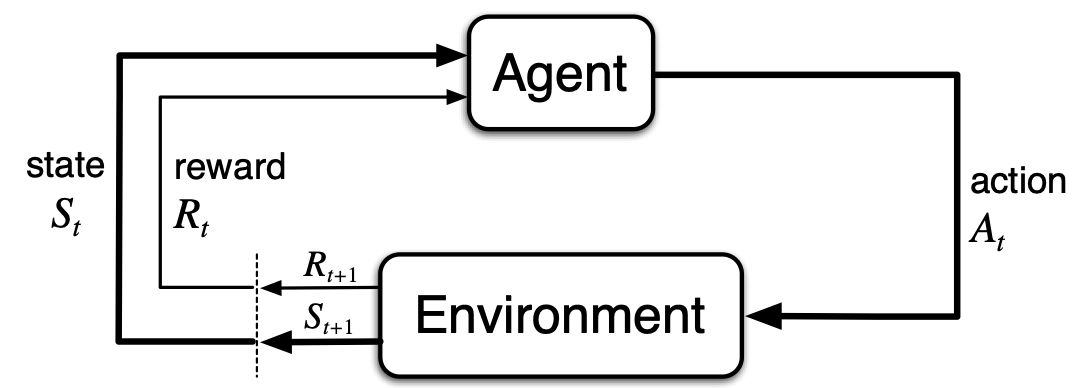
\includegraphics[width=0.5\textwidth]{Figures/agent_environment_model.png}
\caption{Schematic illustration of Reinforcement Learning, copied from
\cite{sutton_reinforcement_2018}}
\label{fig:agent_environment_model}
\end{wrapfigure}
Reinforcement Learning is a branch of Machine Learning that aims to train an
agent in a dynamic environment. At each time step $t$, the agent takes an
action $A_t$ based on the observed environment state $S_t$. The
environment reacts by providing a reward signal $R_{t+1} \in \mathbb{R}$. The
goal of the agent is to select its actions in such a way that the sum of
reward signals (called return) is maximized. The action selection strategy is
referred to as policy. A schematic illustration of an interaction
between agent and environment is shown in Figure~\ref{fig:agent_environment_model}.
In our experiments, the action is the choice of speed for
each pump given a state represented by sensor readings,
and the reward is determined by the energy efficiency and satisfactory operating conditions
(see Section~\ref{sec:experimental_setup}).

The Soft Actor-Critic algorithm (SAC)
\cite{haarnoja_soft_2018} has
particularly promising properties for the pump scheduling task: It was
designed to handle large and continuous action spaces, which makes it a good
candidate for the simultaneous control of multiple variable-speed pumps. SAC
employs a replay buffer, meaning that it stores previous experience to be
re-used in training, which improves data efficiency. A specialty of SAC is the training objective: In
addition to the common RL goal of finding the policy that will maximize the
expected return, a separate term for the maximization
of entropy in the probabilistic policy is introduced.
% \begin{equation}
% J(\pi) = \sum_{t=1}^T \mathbb{E}_{(s_t, a_t) \sim \rho(\pi)} \left[ r(s_t, a_t) +
% \alpha \mathcal{H}(\pi(\cdot | s_t))\right]
% \label{eq:sac_objective}
% \end{equation}
% In Equation ~\ref{eq:sac_objective}, $J$ is the full objective, $\pi$ is the
% policy, $t$ denotes a timestep, and $s$ and $a$ are state and action,
% respectively. The distribution $\rho$ describes the probability of taking
% action $a$ in state $s$ under the current policy. Entropy is denoted by
% $\mathcal{H}$ and $\alpha$ is a weighting factor.
This leads to better exploration behaviour of the agent and more robust
training over all. For a detailed description of SAC, we refer the
interested reader to the original paper \cite{haarnoja_soft_2018} as well as
to the following online resource for an
overview\footnote{\href{https://spinningup.openai.com/en/latest/algorithms/sac.html}{https://spinningup.openai.com/en/latest/algorithms/sac.html}}.

\subsection{Related Work}
\label{sec:related_work}
The operation of pumps in WDNs has been optimized for several decades with
varying techniques and objectives \cite{mala-jetmarova_lost_2017}. A common theme of
existing approaches is the goal of reducing the energy cost of pumping. In
addition, several other constraints and objectives have been treated in the
literature, ranging from pressure bounds at consumer nodes
\cite{hajgato_deep_2020} over control of tank levels \cite{baran_multi-objective_2005} to robustness against leakage events
\cite{giustolisi_operational_2013}.
Traditional methods optimize a fixed pump schedule for a certain
period of time based on a computational model of the WDN and assumptions
on consumer demands \cite{ostfeld_ant_2008}. More recent methods aim to dynamically
adapt the schedule to the current state of the network
\cite{pei_real-time_2025}. RL is particularly promising for this
direction of research, as it models the pump scheduler as an agent in a dynamic
environment, deciding on the next action to apply based on current observations
of the network.
Previous approaches included tabular Q-learning \cite{candelieri_intelligent_2019}, usage of deep networks \cite{hajgato_deep_2020,ma_pump_2024} and scheduling of valves in large distribution networks under uncertainty \cite{belfadil_drl-epanet_2022}.
% A pioneering work by Candelieri \etal \cite{candelieri_intelligent_2019}
% applied tabular Q-Learning \cite{watkins_q-learning_1992}. Following
% approaches used deep networks as function approximators, enhancing the
% scalability to larger networks and more complex observations
% \cite{hajgato_deep_2020,ma_pump_2024}. Belfadil \etal successfully employed RL
% for scheduling of valves in large WDNs under uncertainty
% \cite{belfadil_drl-epanet_2022}.
However, most of the existing literature on
pump control assumes deterministic demands or knowledge of the demand pattern
by the agent. To address a more realistic use case, we evaluate the
performance of the agent under uncertainty. Our goal is to minimize the price
for pumping energy while making sure that the pressure at consumer nodes in
the network stays within acceptable bounds.

The work most closely related to ours is a very recent publication by Pei
\etal \cite{pei_real-time_2025}. The authors optimize an objective similar to
ours taking demand uncertainty into account. The
observations they provide to the agent differ throughout their experiments: In
one setup they assume very limited information comprised only of tank levels
and pump status, while in another they assume knowledge of demand forecasts
for every node in the network. We argue that the former underestimates
available information as knowledge from sensors distributed across the network
is not included while the latter might be an overestimation as demand information may not be available or reliable in the real world. %in cases where
%demand forecasts are only available for a subset of nodes, or the forecasting
%model is not reliable.
In order to further improve the practical use of RL for
pump scheduling, we conduct an in-depth analysis of the benefit of different observation types and different amounts of pressure sensors.

\section{Case Study: Pump Scheduling for Anytown}
\label{sec:experimental_setup}
% info about Net3 and about sensor placement
% and wrappers should go here


We formulate the reward as a weighted sum of two partial rewards
\begin{align*}
r &= c_1 \cdot r_{\text{pres}} + c_2  \cdot r_{\text{energy}} &   \text{s.t.} \quad \ c_1 + c_2 &=
1,\ c_1, c_2 > 0 \\
r_{\text{pres}} &= \frac{1}{N} \sum_{n=1}^N \mathbb{I}(h_{min} <
h[n] < h_{max}) &    r_{\text{energy}} &= 1 - \sum_{p=1}^P \frac{E(p)}{E_{max}(p)}.
\end{align*}
Here, $r_{\text{pres}}$ as in \cite{hajgato_deep_2020} measures the agent's
ability to satisfy pressure constraints at consumer nodes, 
where $\mathbb{I}$ is the indicator function, $h[n]$ is the pressure at node
$n$ and $h_{min}, h_{max}$ are lower and upper pressure constraints,
respectively.
The second term, $r_{\text{energy}}$, reflects the energy consumption of the
pumps, where $E(p)$ is the energy consumption of pump $p$ and $E_{max}(p)$ is its
maximum energy consumption, determined empirically before optimization.
To ensure constraint satisfaction, we used weights of $c_1=0.9$ and
$c_2=0.1$ throughout the experiments. The action of the agent is a vector of
relative speed settings, ranging from 0 to 1 for each pump in the network. To investigate the effects on performance, we trained the agent with different sensory information in the current state. The configurations used are described
in Tab.~\ref{tab:state_acronyms}
\begin{table}[htb]
\centering
\begin{tabular}{l|c|c|c|c|c}
    \textbf{Acronym} & \textbf{Tank-Level} & \textbf{Daytime} & \textbf{Pressure} & \textbf{Flow} & \textbf{Energy Consumption}\\
    \hline
    TD & \cmark & \cmark & \xmark & \xmark & \xmark \\
    TP(A) & \cmark & \xmark & all nodes & \xmark & \xmark \\
    TDP(A) & \cmark & \cmark & all nodes & \xmark & \xmark \\
    TDP(1) & \cmark & \cmark & one random node & \xmark & \xmark \\
    TDP(8) & \cmark & \cmark & eight random nodes & \xmark & \xmark \\
    TDP(A)FE & \cmark & \cmark & all nodes & \cmark & \cmark
\end{tabular}
\caption{Acronyms of different state representations used during training}
\label{tab:state_acronyms}
\end{table}
To conduct our experiments, we used the SAC implementation of Stable Baselines
3 \cite{raffin_stable_2021} with default hyperparameters with the following exceptions: 
We increased the learning rate to $3 \cdot 10^{-3}$ and fixed the entropy
coefficient to $10^{-2}$.
For our case study, we used a variant of the Anytown network
\cite{walski_battle_1987} as used in
\cite{reis_cost-efficient_2024}. The network contains three pumps connected to the reservoir, which supplies water to 19 junctions, connected by 42 pipes. Three
storage tanks are installed as water buffers. The network file and our code
are publicly available\footnote{Link to code and data on GitHub:
\href{https://github.com/HammerLabML/RL4Water\_Sensor\_Placement\_Anytown}{https://github.com/HammerLabML/RL4Water\_Sensor\_Placement\_Anytown}}.
Following the general guidelines for pressure constraints in water networks
\cite{ghorbanian_pressure_2016}, we used a lower pressure constraint of 28.12m and an upper constraint of 70m. We utilized the EPANET simulator
\cite{rossman_epanet_2020} through the EPyT-Flow Python library
\cite{artelt_epyt-flow_2024}. Experiments used a 30min
time step for a duration of 24 hours. Due to stochasticity in the training
process, we repeated each training run five times using different seeds and averaged the results. This includes different sensor placements for the random locations. To
test the agent's ability to generalize to unseen scenarios, we added 5\% of
uncertainty to the demand pattern at each node. To account for this
uncertainty, the results reported below in Table~\ref{tab:rewards} were
additionally averaged over ten 24-hour episodes.

\section{Results and Discussion}
\label{sec:results_and_discussion}
\begin{figure}[htb]
    \centering
    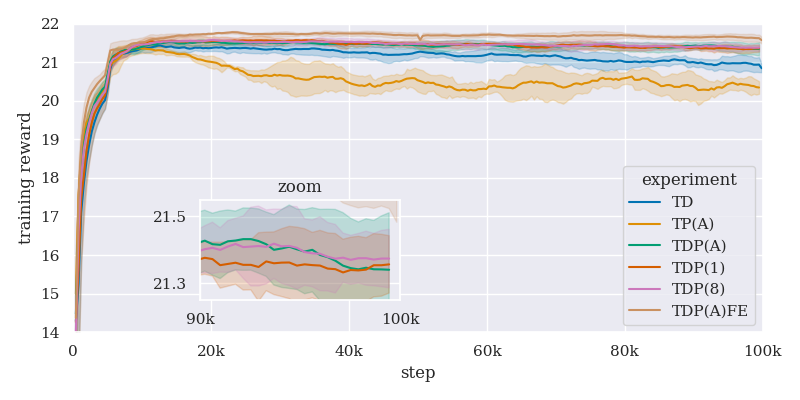
\includegraphics[width=0.75\linewidth]{Figures/rewards_zoom.png}
    \caption{The training reward during the training process. The shaded area represents the standard deviation over the five repetitions. The lines of the different pressure sensor configurations are included in a zoomed in window, since they overlap heavily.}
    \label{fig:reward_training}
\end{figure}



The episodic returns over the course of all  training runs are depicted in Fig. \ref{fig:reward_training}.
The plotted results reveal, that all observation types are beneficial for the agent to reach a higher reward.
However, while adding pressure values to the observation in general results in a clearly visible improvement, the amount of sensors matters relatively little.
The reward curves are nearly indistinguishable from one another. Furthermore
the standard deviation is small in comparison between the experiments \textit{TD} and \textit{TP(A)}, so the curves are similar regardless of the random sensor locations.

% \begin{table}
%     \centering
%     \begin{tabular}{l|c|c|c}
%          Experiment & Pressure & Price & Smoothness\\
%          \hline
%          TD & $0.999 (.018)$ & $0.607 (.159)$ & $0.940 (.055)$\\
%          TP(A) & $0.999 (.009)$ & $0.588 (.164)$ & $0.951 (.043)$\\
%          TDP(A) & $1.000 (.011)$ & $0.606 (.172)$ & $0.947 (.060)$\\
%          TDP(1) & $0.999 (.012)$ & $0.602 (.173)$ & $0.932 (.073)$\\
%          TDP(8) & $\mathbf{1.000 (.005)}$ & $0.596 (.153)$ & $\mathbf{0.961 (.049)}$ \\
%          TDP(A)FE & $\mathbf{1.000 (.005)}$ & $\mathbf{0.652 (.261)}$ & $0.667 (.214)$\\
%     \end{tabular}
%     \caption{This table lists the mean partial rewards the agents reached after training per time step. The standard deviation is given in parentheses.}

%     \label{tab:rewards}
% \end{table}

\begin{wraptable}[12]{r}{65mm}
    \begin{tabular}{l|c|c}
         Experiment & Pressure & Price \\
         \hline
         TD & $0.999 (.018)$ & $0.607 (.159)$\\
         TP(A) & $0.999 (.009)$ & $0.588 (.164)$\\
         TDP(A) & $1.000 (.011)$ & $0.606 (.172)$\\
         TDP(1) & $0.999 (.012)$ & $0.602 (.173)$\\
         TDP(8) & $\mathbf{1.000 (.005)}$ & $0.596 (.153)$\\
         TDP(A)FE & $\mathbf{1.000 (.005)}$ & $\mathbf{0.652 (.261)}$\\
    \end{tabular}
    \caption{This table lists the mean partial rewards the agents reached after training per time step. The standard deviation is given in parentheses.}
    \label{tab:rewards}
\end{wraptable}

For a more detailed look into the performance of the fully trained agents we refer to Tab. \ref{tab:rewards}.
The table splits the reward into its components of keeping all nodes within pressure bounds and optimizing the operation costs of the pumps.
All agents have managed to find a policy to stay within the pressure bounds at all nodes with only small deviations.
The price objective gains another noticable boost from the added flow and energy consumption information.
However, while inspecting the policy over the course of one day, we found that
the agent gained that boost by learning to switch the pump on and off every
other hour. Using an additional reward term to discourage this behaviour is
part of our ongoing research.
%Hence, we added a third column, which evaluates the smoothness of the learned policies, ensuring no overly large changes within the last three steps.
%All other agents do not follow a disruptive pattern like that.


%The similar performances of different pressure sensors show that sparse sensor placements are sufficient to factor in pressure for pump schedule optimization.
%It remains an open question how this scales to larger networks, where pressure will be more varied over nodes and sensor locations may become more important.
%While we started experimenting with larger networks, some of the problems we encountered were uncertainty of whether all pressure bounds could be fulfilled, instable hydraulic states during exploration and runtime.

\section{Conclusion}
\label{sec:conclusion}
While \cite{pei_real-time_2025} have achieved good results using only tank
levels and pump speeds, we show that it is beneficial to include other sensor
information that can be available in real world scenarios such as pressure
sensors. Enforcing limited pump switch to improve applicability remains a
challenge for future work.
%However, as is well-known in the RL community, agents can learn unfeasible policies in simulated environments. Hence, it is important to check the applicability of the learned policies to real life, e.g. no quick succession of switches in the pump states.
%Building on our experiments we plan to extend our research to bigger networks and sparser but more deliberate sensor configurations.

\section{Acknowledgments}
\label{sec:acknowledgments}
We gratefully acknowledge funding from the European Research Council (ERC)
under the ERC Synergy Grant Water-Futures (Grant agreement No. 951424). We are
thankful for the support of Andr\'e Artelt, maintainer of EPyT-Flow, who
implemented various feature requests to make this work possible.



\printbibliography
\end{document}
